\documentclass{article}
\usepackage[utf8]{inputenc}

\usepackage[letterpaper, margin=1in]{geometry}
\usepackage{amsmath}
\usepackage{enumitem}
\usepackage{caption}
\usepackage{subcaption}
\usepackage{graphicx}
\graphicspath{ {figures/} }

\title{Analytical analysis of a pedestrianized corridor in the center of a rectilinear city}
\author{Nicholas Fournier}
\date{February 2020}

\begin{document}


\maketitle



Consider an idealized city of dimension $R$ with a rectilinear street network with spacing $S$ and a pedestrianized central corridor of length $\gamma$, as shown in Figure~\ref{fig:gridcity}. The pedestrianized corridor blocks all traffic moving longitudinally, but allows traffic to cross perpendicularly. Trips generated by the area around the pedestrianized zone must now be diverted to neighboring streets, adding to existing flow.

\begin{figure}[!ht]
     \centering
     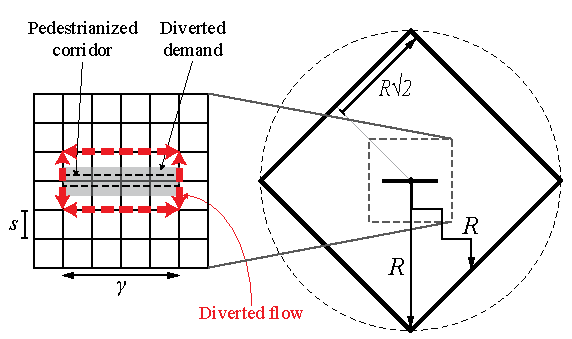
\includegraphics[width=0.5\textwidth]{diagram_grid_city}
     \caption{Rectilinear city with pedestrianized corridor}
     \label{fig:gridcity}
\end{figure}

\noindent The objective is to evaluate the traffic impact on the parallel streets. Specifically,

\begin{enumerate}[topsep=3pt, itemsep=3pt, partopsep=3pt, parsep=3pt]
    \itshape
    \item what capacity is required by the parallel streets and
    \item what are the impacts on travel time?
\end{enumerate}

\noindent Traffic flow through the network is characterized by the macroscopic fundamental diagram (see Figure~\ref{fig:mfd}) with travel time cost (see Figure~\ref{fig:traveltime}):

\begin{figure}[!ht]
     \centering
     \hfill
     \begin{subfigure}[b]{0.4\textwidth}
         \centering
         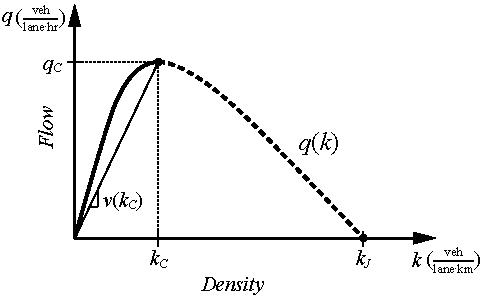
\includegraphics[width=\textwidth]{diagram_mfd}
         \caption{Macroscopic fundamental diagram}
         \label{fig:mfd}
     \end{subfigure}
     \hfill
     \begin{subfigure}[b]{0.4\textwidth}
         \centering
         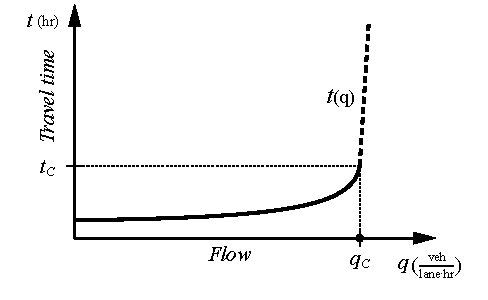
\includegraphics[width=\textwidth]{diagram_traveltime}
        \caption{Macroscopic fundamental diagram}
         \label{fig:traveltime}
     \end{subfigure}
     \hfill
     \caption{Macroscopic fundamental diagram and travel time cost function}
\end{figure}

The travel time cost function depending on traffic flow and density can be defined as

\begin{align}
    t(q) &= l \frac{k(q)}{q} & \text{for}~q < \mu \\
    t(q) &= t_c (\frac{q}{\mu})  & \text{for}~q \geq \mu
\end{align}

\noindent where $t(q)$ is travel time for flow $q$, $k(q)$ is traffic density for flow $q$, $l$ is link length, and $\mu$ is link capacity. Assuming for this case a parabolic function for the uncongested portion of the flow-density relationship, an expression can be written as

\begin{equation}
    q(k) = q_c - (\beta k - k_c)^2
\end{equation}

\noindent where $k_c$ is the density at capacity, $q_c$ is the flow at capacity, and $\beta$ is a fitting parameter. In order to determine travel time using density as a function of flow, $k(q)$, it can be solved for using the quadratic formula

\begin{equation}
    k(q) = \frac{k_c - \sqrt{q_c - q^*}}{\beta}
\end{equation}

\noindent where $q^*$ is the calculated peak flow required along the parallel streets.

Demand is generated in the city area in units of $\frac{trips}{dist^2}$, and can be simplified into two types: 

\begin{itemize}[topsep=3pt, itemsep=3pt, partopsep=3pt, parsep=3pt]
    \item Uniform baseline travel across the network, $\lambda_b$, and
    \item Monocentric travel demand going to and from the center of the city, $\lambda_c$
\end{itemize}

The flow at a point $r$ distance from the city center is then the summation of this baseline demand and the monocentric demand, calculated as:

\begin{equation}
    q(r) = \frac{\lambda_b R}{\delta} + \frac{\lambda_c}{4r\delta} \left( \frac{R^2}{r} - r \right)
\end{equation}

\noindent where $\delta$ is the street density in $\frac{lane \cdot dist}{dist^2}$, calculated as $\delta = \frac{4S}{S^2} = \frac{4}{S}$. The critical flow, $q^*$, along parallel streets is then calculated as the flow of trips that would otherwise use the parallel streets, $q(r=s)$, plus the flow diverted to the parallel streets from the street closure.

\begin{equation}
    q^* = \frac{\lambda_b R S}{4} + \frac{\lambda_c}{16} \left( \frac{R^2}{S} - S \right) + \gamma S (\lambda_b + \lambda_c)
\end{equation}

\end{document}
